Avant même d'aborder les fonctionalités graphiques de R, vous devons préciser qu'elles sont quasi infinies. C'est donc pour cette raison que nous nous contenterons de ne faire qu'une revue globale des types de graphiques qui combleront amplement vos besoins pour faire vos premiers pas. Advenant le cas où ces connaissances ne seront plus suffisantes, il existe énormément d'exemples sur les forums de la communauté pour appeser votre curiosité. \\

\noindent
Pour débuter, la fonction \emph{plot} est de loin la fonction la plus rudimentaire de faire un graphique avec R. Cette fonction ne possède que trois arguments: \texttt{x}, \texttt{y} et \texttt{...}. Naturellement, nous devrons fournir des valeurs d'abscisse et d'ordonnée à la commande \emph{plot} via les arguments \texttt{x} et \texttt{y} et la fonction s'occupera de produire un graphique à points traditionnel. En partant directement du jeu de données \emph{airports.dat}, nous pouvons être tentés d'essayer cette commande en représentant les couples longitude/latitude de chaque aéroport dans le monde. Bien entendu, le résultat obtenu sera peu élégant ne représentant que l'essentiel. \\

\noindent
C'est à ce moment que l'argument \texttt{...} entre en scène. Nous n'avons pas discuter de ce type d'argument dans la section précédente puisque nous considérions plus intuitif de le présenter à l'aide d'un exemple de son utilisation la plus commune, le passage d'options graphiques au sein de la commande \emph{plot}. Il ne sera toutefois pas rare de retrouver cet argument dans bon nombre de fonction, mais sa nécessité sera souvent moindre que dans le cas de la création de graphique. Cet argument possède la propriété particulière d'absorber tous les paramètres qui seront passés à la fonction et qui n'auront pas été assignés à un argument. Ces mêmes paramètres pourront donc ensuite être transmis à une autre fonction au sein du corps de la fonction. \\

\noindent
C'est exactement ce qui se produit dans le cas de la commande \emph{plot} qui enverra tous les paramètres supplémentaires à la commande \emph{par} étant la commande gérant tous les aspects des graphiques en R. Heureusement, il existera des comportements par défaut pour tous les arguments de cette fonction et puisqu'il sera inconcevable et surtout inutile à quiconque d'apprendre l'ordre réel dans lequel ces arguments se présentent, le passage des paramètres se fera en nommant chaque argument sur lequel nous voulons imposer un comportement différent. C'est précisément ce que nous avons fait dans la deuxième version de notre graphique (\autoref{fig:LonLatMap}) en spécifiant le nom des axes (\emph{xlab} et \emph{ylab}) ainsi qu'un titre au graphique (\emph{main}). Nous avons aussi modifié le type de point pour passer de points vides à des points remplis (\emph{pch}) tout en réduisant la taille de ces dernier pour obtenir une meilleure résolution (\emph{cex}). Finalement, nous avons utilisez une police en gras pour le titre du graphique et les axes (\emph{font} et \emph{font.lab}) en plus de venir augmenter la taille de ces derniers (\emph{cex.main} et \emph{cex.lab}). Référez-vous au \autoref{src:plot} pour plus de détails. \\
	
\begin{figure}
	\begin{minipage}{\textwidth}
		\centering
		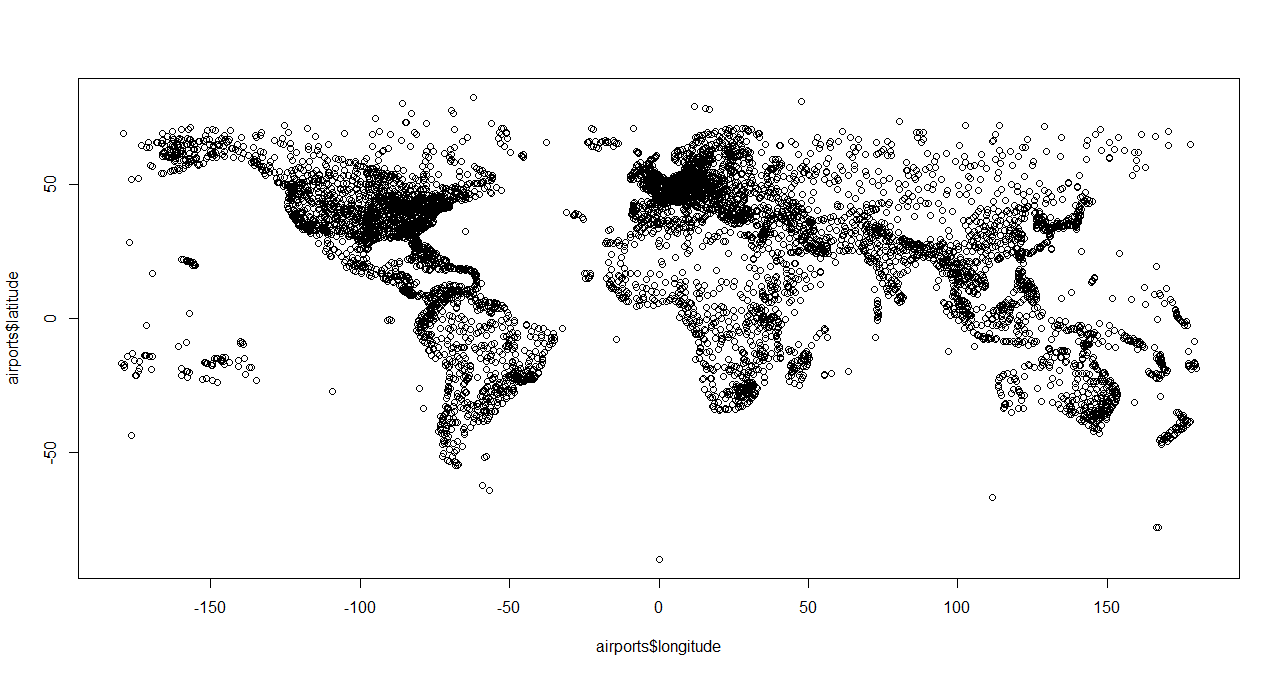
\includegraphics[width=\textwidth, height=\textheight,keepaspectratio]{LonLatMapV1}
	\end{minipage}
	\newline
	\begin{minipage}{\textwidth}
		\centering
		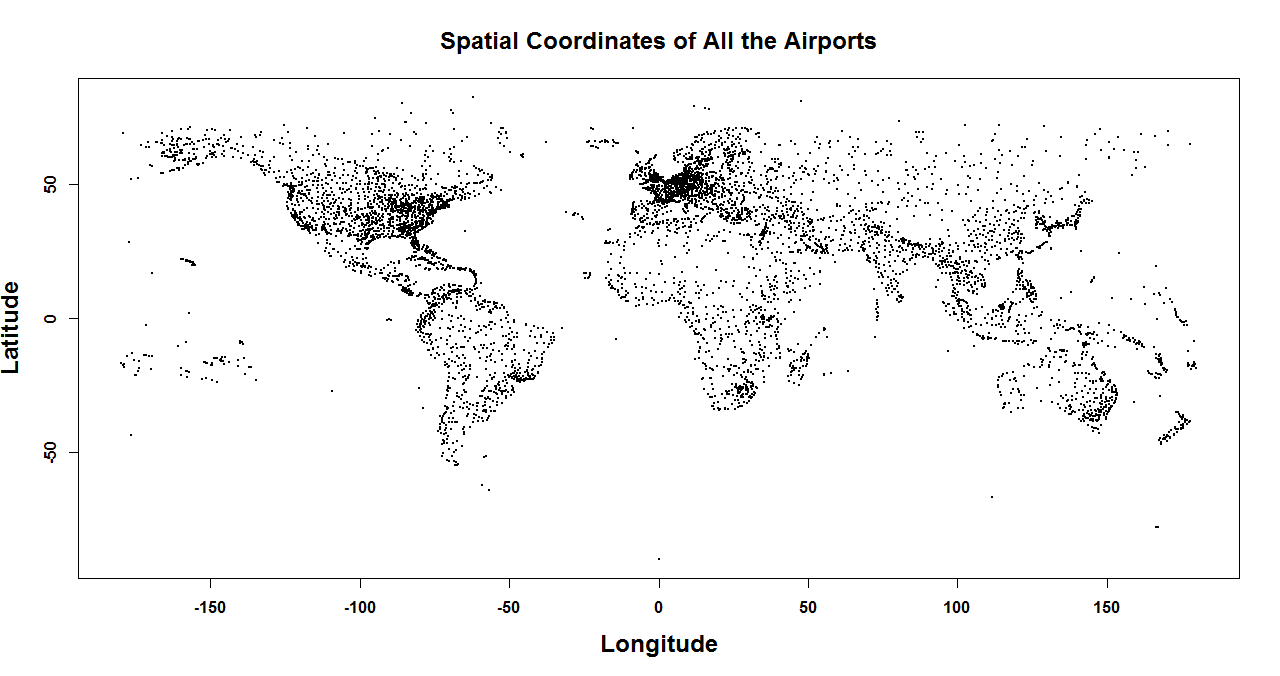
\includegraphics[width=\textwidth, height=\textheight,keepaspectratio]{LonLatMapV2}
	\end{minipage}
	\caption{Passage de paramètres graphiques à la commande \emph{plot}}
\end{figure}
\label{fig:LonLatMap}

\begin{lstlisting}[caption = Utilisation de la commande \emph{plot},label=src:plot]
plot(airports$longitude,airports$latitude)
plot(airports$longitude,airports$latitude,cex = 0.1,xlab="Longitude",ylab="Latitude",main="Spatial Coordinates of All the Airports",pch = 20,font = 2,cex.main = 1.5,font.lab = 2,cex.lab = 1.5)
\end{lstlisting}

\vspace{\baselineskip}
\noindent
Dans le cas où nous aurions plutôt voulu faire la représentation d'une fonction continue, nous pourrions encore une fois utiliser la commande \emph{plot} en modifiant l'argument \emph{type}. Bien que cette pratique peut nous sembler justifiée, elle pourra jouer de mauvais tours à un utilisateur non-averti. Comme le montre la \autoref{fig:plotCurve}, dépendemment de l'espacement des valeurs points caculés, nous pourrions perdre toute l'information sur l'allure réelle de la courbe que nous cherchons à visualiser. \\

\noindent
Il sera donc préférable d'utiliser la commande \emph{curve} pour ce genre de tâche afin de simplifier le code source en ne précisant que les extrêmes de l'étendu sur lequel nous voulons tracer la fonction en spécifiant au besoin le nombre de valeur à calculer dans l'intervalle. \\

\begin{lstlisting}[caption = Utilisation de la commande \emph{curve},label=src:plotCurve]
fquad <- function(x,a=2,b=3,c=4)
{
  a*x**2+b*x+c
}
fquad(2)
par(mfrow = c(2,2))
plot(x <- seq(-10,10,10),fquad(x,2,3,4),type = "l",ylab = "fquad(x)",xlab = "x",main = "dx = 10")
plot(x <- seq(-10,10,5),fquad(x,2,3,4),type = "l",ylab = "fquad(x)",xlab = "x",main = "dx = 5")
plot(x <- seq(-10,10,2),fquad(x,2,3,4),type = "l",ylab = "fquad(x)",xlab = "x",main = "dx = 2")
plot(x <- seq(-10,10),fquad(x,2,3,4),type = "l",ylab = "fquad(x)",xlab = "x",main = "dx = 1")

par(mfrow = c(1,1))
curve(fquad(x),from = -10,to = 10)
\end{lstlisting}

\addPicture{1}{0.5}{plotCurve}{Tracer une courbe avec la commande \emph{plot}}{plotCurve}

\addPicture{1}{0.5}{curve}{Tracer une courbe avec la commande \emph{curve}}{curve}

